\section{Responsive Design}
The use of mobile devices for internet browsing has grown at an astronomical pace, but unfortunately, much of the web is not optimised for mobile device usage. Mobile phones are often constrained by display size and require a different approach to how content is laid out on screen \cite{GoogleDev:Responsiveness}. Since the introduction of CSS media queries and frameworks such as Bootstrap, responsive web applications are becoming an ever increasing sight given to their ability to serve multiple devices \cite{Bootstrap:Home}. Before we delve into the Bootstrap framework and its column layout it is important to understand what media queries are and how they work, as custom media queries are used throughout the application. Pete LePage, a web development advocate, described media queries as ``simple filters that can be applied to CSS styles. They make it easy to change styles based on the characteristics of the device rendering the content, including the display type, width, height, orientation and even resolution." \cite{GoogleDev:Responsiveness}.

Bootstrap easily and efficiently scales websites and applications with a single code base, from phones to desktops by employing media queries \cite{Bootstrap:Home}. In order to achieve this, Bootstrap implements a responsive, mobile first fluid grid system that appropriately scales up to 12 columns as the device or viewport size increases \cite{Bootstrap:Grid}.

\begin{figure}[H]
\centering
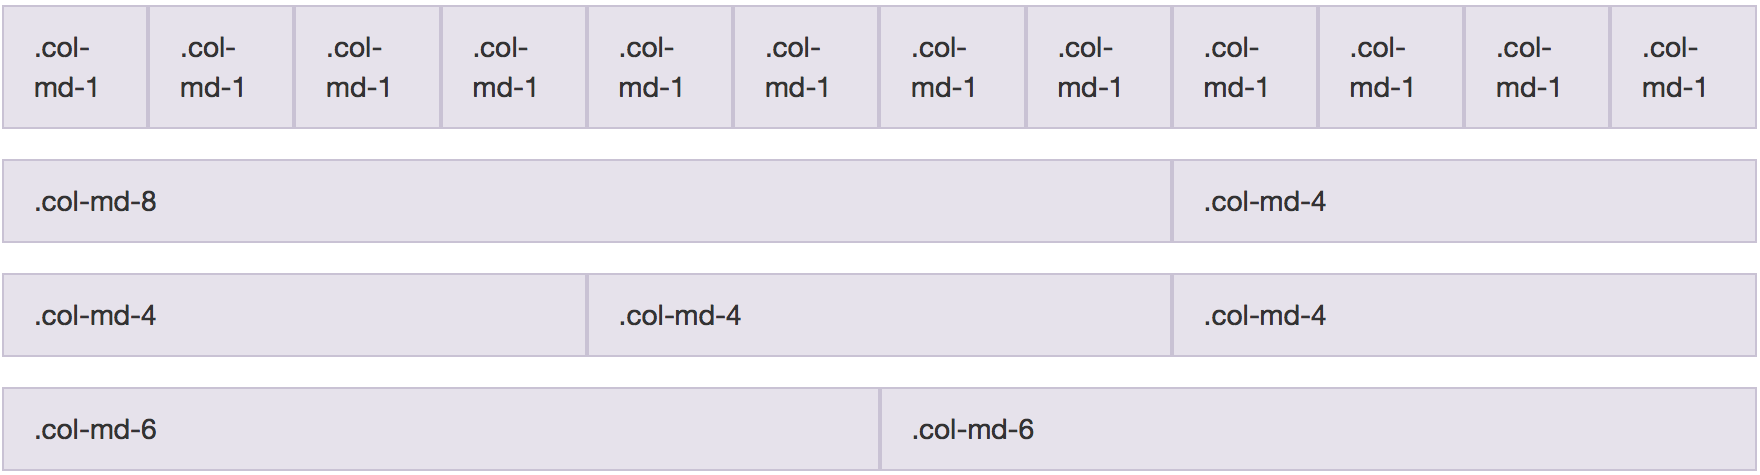
\includegraphics[width=1.0\textwidth]{Images/Implementation/BootstrapGrid}
\caption{Bootstrap Responsive Grid Example} 
\label{fig:BootstrapGrid}
\end{figure}

The grid system works by using a series of rows and columns, where a row consists of 12 columns. A row is placed within a \emph{.container} or \emph{.container-fluid} for proper alignment. Content is placed within columns which can be sized differently for varying resolutions. Figure \ref{fig:BootstrapGrid} shows the grid system where the first row has 12 elements of \emph{.col-md-1}, which means that on a medium size screen each element will take up one column each, whereas the second row has two elements, the first being 8 columns wide and the second only 4 columns wide. All these elements specify only column sizes for medium-size screens but these are automatically cascaded to larger screens. However, on a screen size that is smaller than `medium', the elements will each span 12 column and stack vertically. 

\begin{figure}[H]
\centering
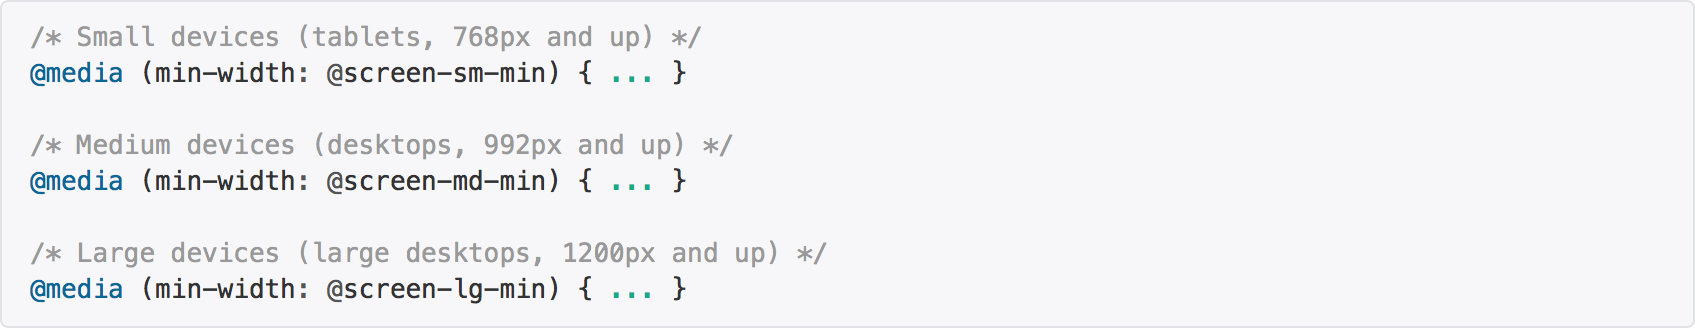
\includegraphics[width=1.0\textwidth]{Images/Implementation/MediaQueries}
\caption{Bootstrap Media Queries for Different Screen Sizes} \label{fig:MediaQueries}
\end{figure}

Figure \ref{fig:MediaQueries} shows the media queries used by bootstrap to achieve the functionality provided by the grid. Each class is defined separately for each screen size inside the query. The grid layout was used throughout the entire website and all content was placed inside columns to ensure that it would be presented correctly on each device.

Through the use of custom media queries, the Bootstrap grid system, and other CSS techniques, an entirely different experience was implemented for devices with different screen sizes. Figure \ref{fig:MobileView} shows the home and profile pages as viewed on a mobile phone.

\begin{figure}[H]
    \centering
    \begin{subfigure}[t]{0.45\textwidth}
        \centering
        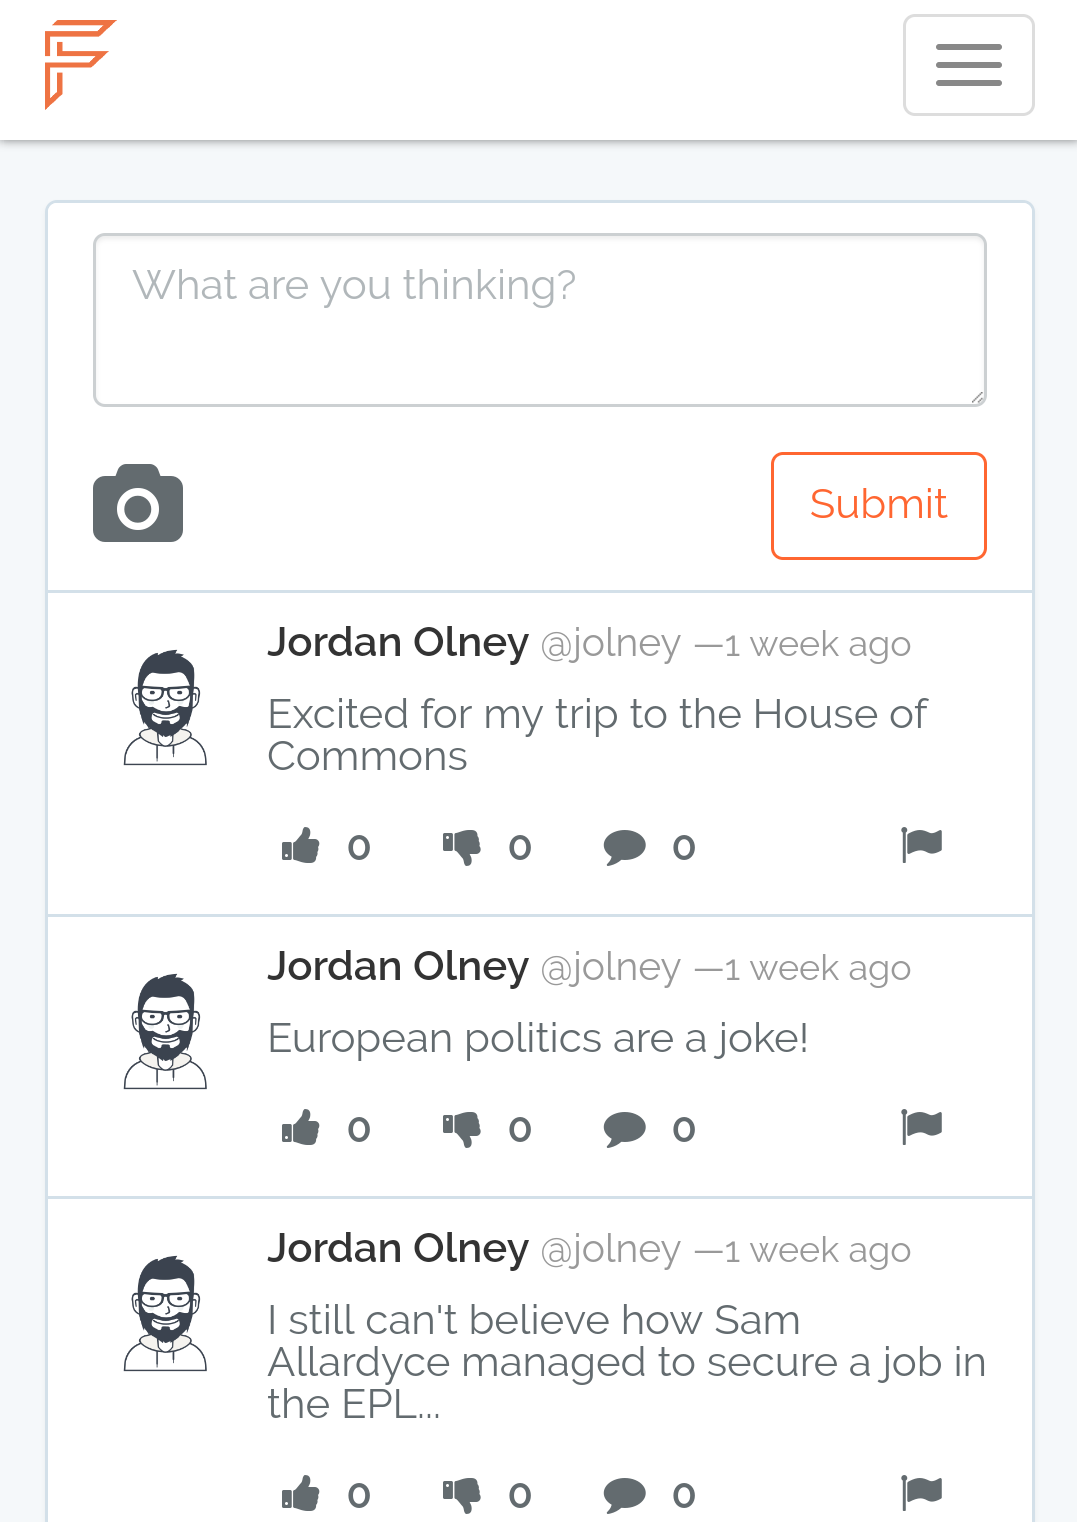
\includegraphics[height=2.5in]{Images/Implementation/MobileHome}
        \caption{Home for mobile}\label{fig:MobileHome}        
    \end{subfigure}
    \quad
    \begin{subfigure}[t]{0.45\textwidth}
        \centering
        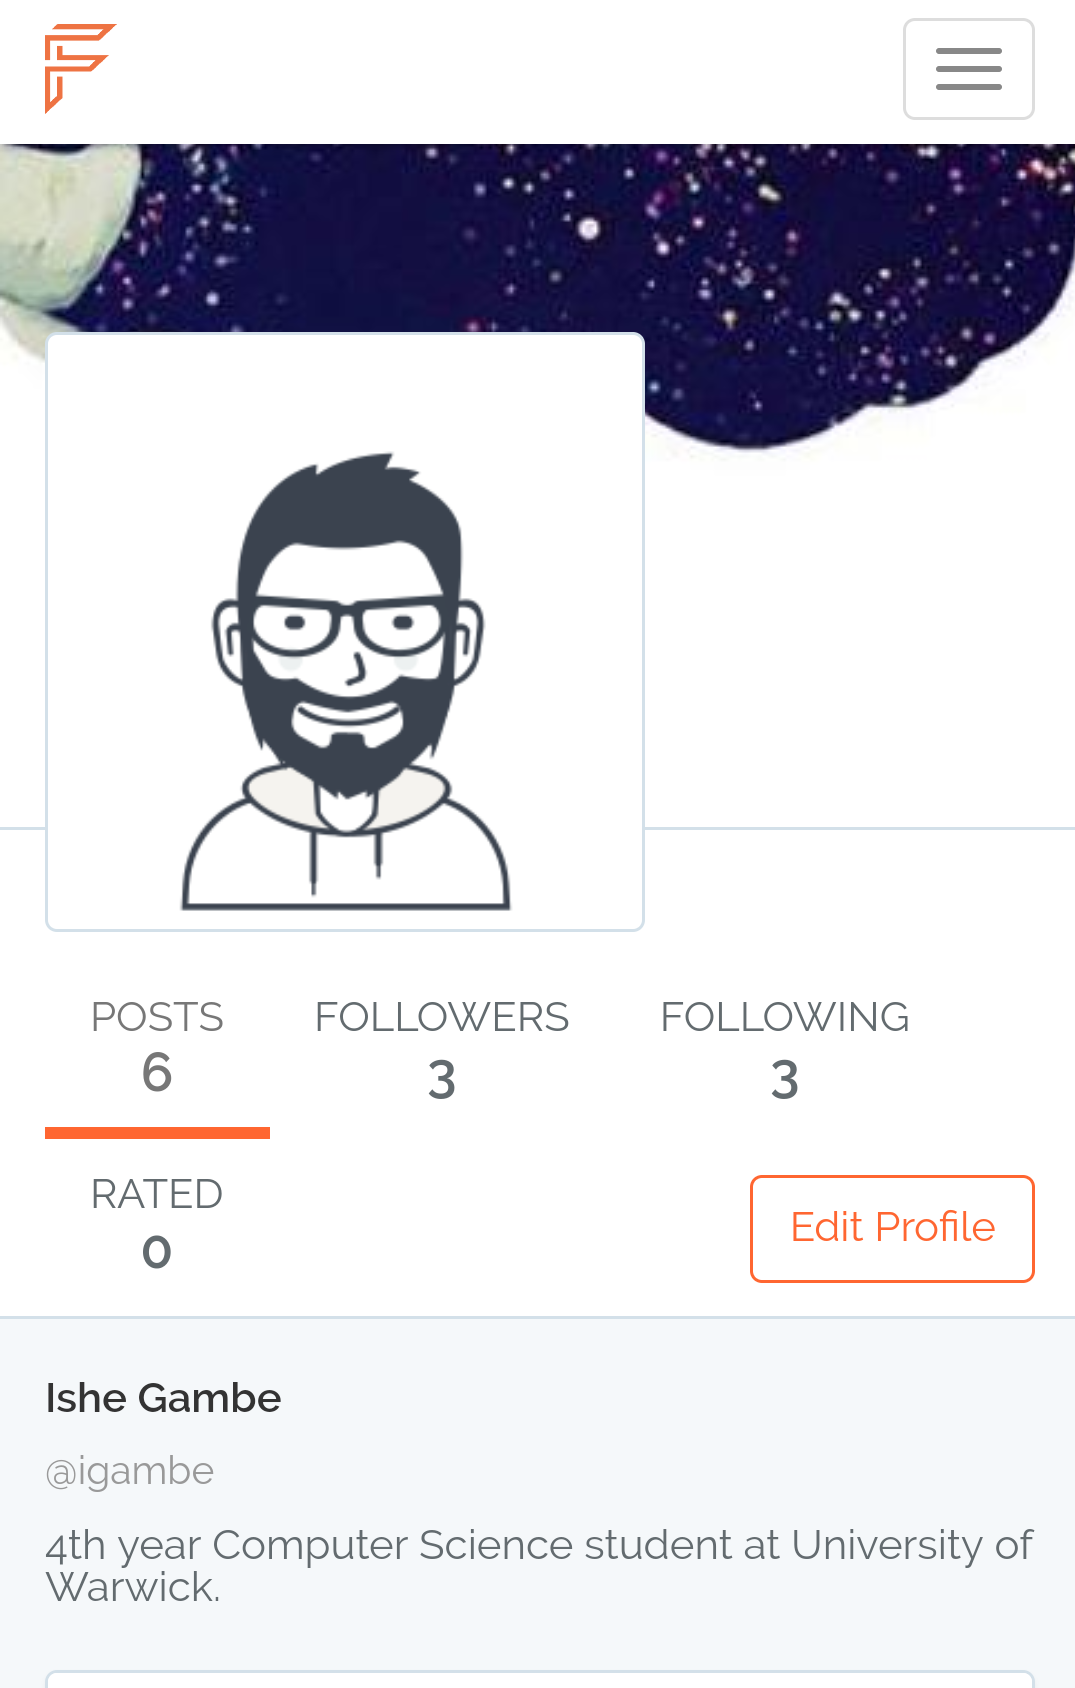
\includegraphics[height=2.5in]{Images/Implementation/MobileProfile}
        \caption{Profile for mobile}\label{fig:MobileProfile}
    \end{subfigure}
    \caption{Mobile versions for (a) home and (b) profile page}\label{fig:MobileView}
\end{figure}